\documentclass{article}

\usepackage[hidelinks]{hyperref}
\usepackage[italian, main=english]{babel}
\usepackage{listings}
\usepackage{xcolor}
\usepackage{microtype}
\usepackage{graphicx}
\usepackage[a4paper, top=2.5cm, bottom=2.5cm, left=2.5cm, right=2.5cm]{geometry}
\usepackage[T1]{fontenc}
\usepackage{lmodern}

\lstset{
    language=Python,
    basicstyle=\ttfamily\small,
    keywordstyle=\color{blue}\bfseries,
    stringstyle=\color{green!50!black},
    commentstyle=\color{gray}\itshape,
    numberstyle=\tiny\color{gray},
    numbers=left,
    stepnumber=1,
    showstringspaces=false,
    breaklines=true,
    frame=single,
    captionpos=b,
    tabsize=4
}

\begin{document}

\begin{titlepage}
    \centering
    \vspace*{2cm}

    
\includegraphics[width=0.4\textwidth]{images/logo_univr.png}\par\vspace{1cm}

    {\scshape\LARGE Università degli Studi di Verona \par}
    \vspace{0.5cm}
    {\scshape\Large Department of Computer Science \par} 
    \vspace{2cm}

    {\Large Internal Internship Project Report\par}
    \vspace{0.5cm}
    
    {\huge\bfseries Skill Gap Evaluation\\[0.3cm] and Course Recommendations \par}
    
    \vspace{2.5cm}

    {\Large\textbf{Author:}\\ Simone Pedretti \\ \large Student ID: VR500040 \par}
    
    \vspace{1cm}

    \vfill

    {\large Academic Year 2025/2026 \par} 
\end{titlepage}

\tableofcontents

\newpage

\section{Introduction}
This report details the work carried out during my internal internship at 
\foreignlanguage{italian}{\textit{Università degli Studi di Verona}}. 
The primary objective of this project was the design and development of a web-based 
platform tailored for skill management, competence tracking, and course recommendation.

From a technical perspective, the application follows a standard client-server 
architecture, with a clear separation of concerns between the frontend and the backend. 
The backend system, hosted on the server to handle the core business logic and data 
management, was developed in Python utilizing the \textbf{FastAPI} framework. 
It heavily relies on the \textbf{JSON} format for efficient data structuring 
and API communication. 
The frontend system, on the client side, was implemented using standard web 
technologies, specifically \textbf{HTML} and \textbf{CSS}. This ensures 
a clean, responsive, and accessible experience for both individual users and 
organizational profiles interacting with the system.

The following sections will provide a detailed overview of the specific features implemented for the 
different types of users, detailing the browsing capabilities, profile management, 
and the skill gap evaluation mechanisms. Furthermore, the report will explore 
the underlying technical components that power these functionalities: 
final chapters will discuss the integration of the \textbf{ESCO API} for standardized 
competence mapping, the strategies adopted for data management, and finally, the testing procedures conducted to 
ensure the reliability and robustness of the system.

\newpage

\section{Individual User Features}
This section outlines the functionalities available to individual users interacting 
with the platform. Within this system, a user can hold one of two distinct roles: 
a standard Employee or a Manager. While an Employee utilizes the platform primarily 
for personal skill tracking and career development, a Manager is a user who has been 
elevated to this status by their affiliated organization. Managers inherit all standard 
employee capabilities but are additionally granted administrative privileges to 
oversee projects and coordinate team members within their company.

\subsection{Home}
The Home dashboard serves as the primary entry point for users, offering intuitive 
search and management tools depending on their assigned role.

\subsubsection{Browsing for Roles and Skills}
Users can explore various professional profiles through the role browsing feature. 
This search mechanism integrates the ESCO API, ensuring that role definitions, 
responsibilities, and terminologies are standardized and perfectly aligned with 
the European labor market classifications.

Similarly to the role search, users can browse for individual competencies. 
By querying the ESCO API, the system retrieves a list of macthing skills. 
This allows users to accurately identify specific 
abilities.

\begin{figure}[htbp]
    \centering
    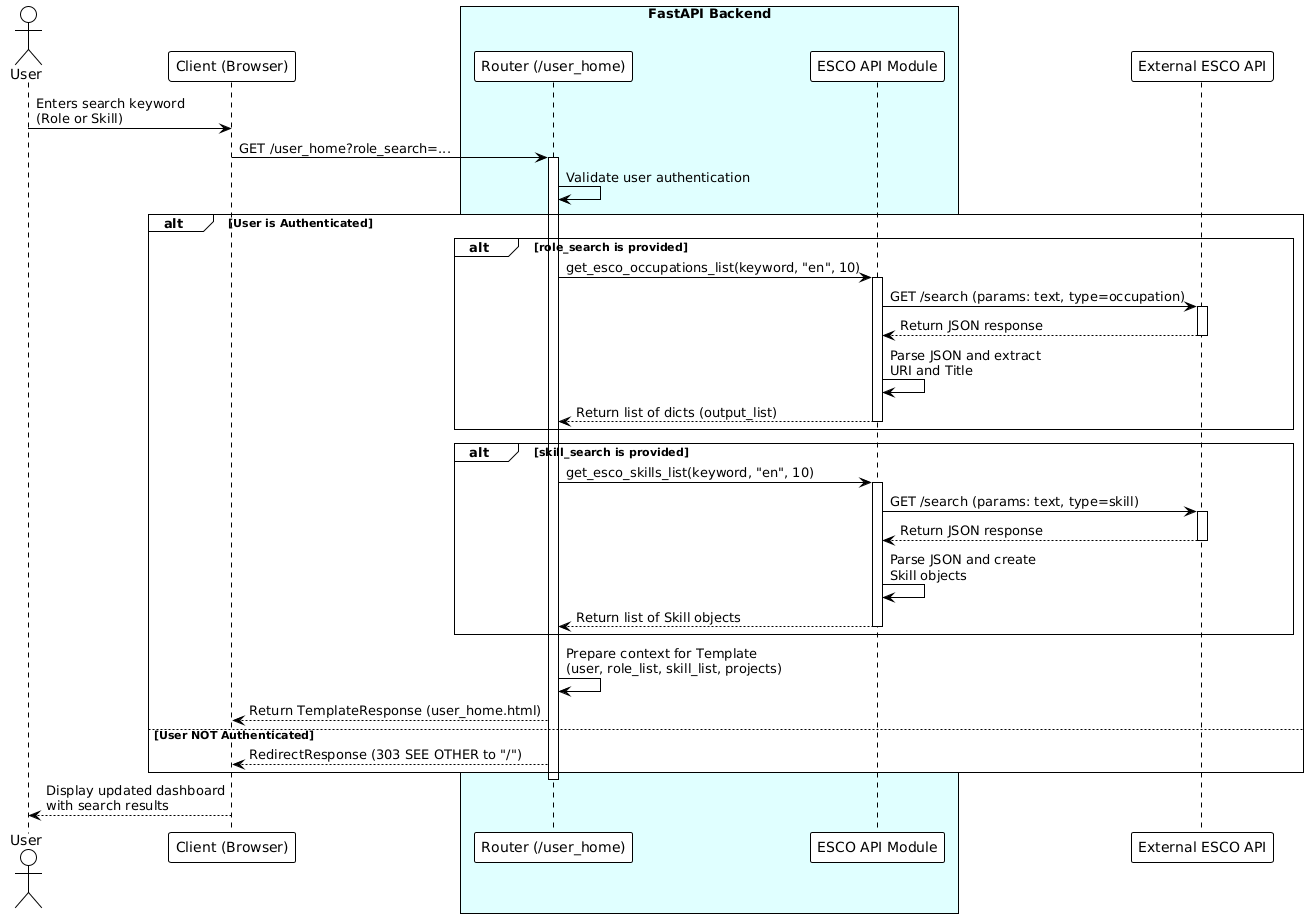
\includegraphics[width=1\linewidth]{images/sequence_diagram_user_esco_api.png}
    \caption{Sequence Diagram: User - Esco API}
\end{figure}

\subsubsection{Project Manager}
This dedicated area is exclusively accessible to users with Manager privileges. 
Here, managers can create, organize, and oversee various internal projects. 
They have the authority to assign team members to these projects, provided those 
individuals belong to the same organization. Furthermore, managers can select specific 
target roles for a project to calculate Cedefop-based employment forecasts and 
generate preliminary course recommendations for the team. A more comprehensive 
explanation of the forecasting and recommendation mechanisms is detailed in the 
Profile section below.

\begin{figure}[htbp]
    \centering
    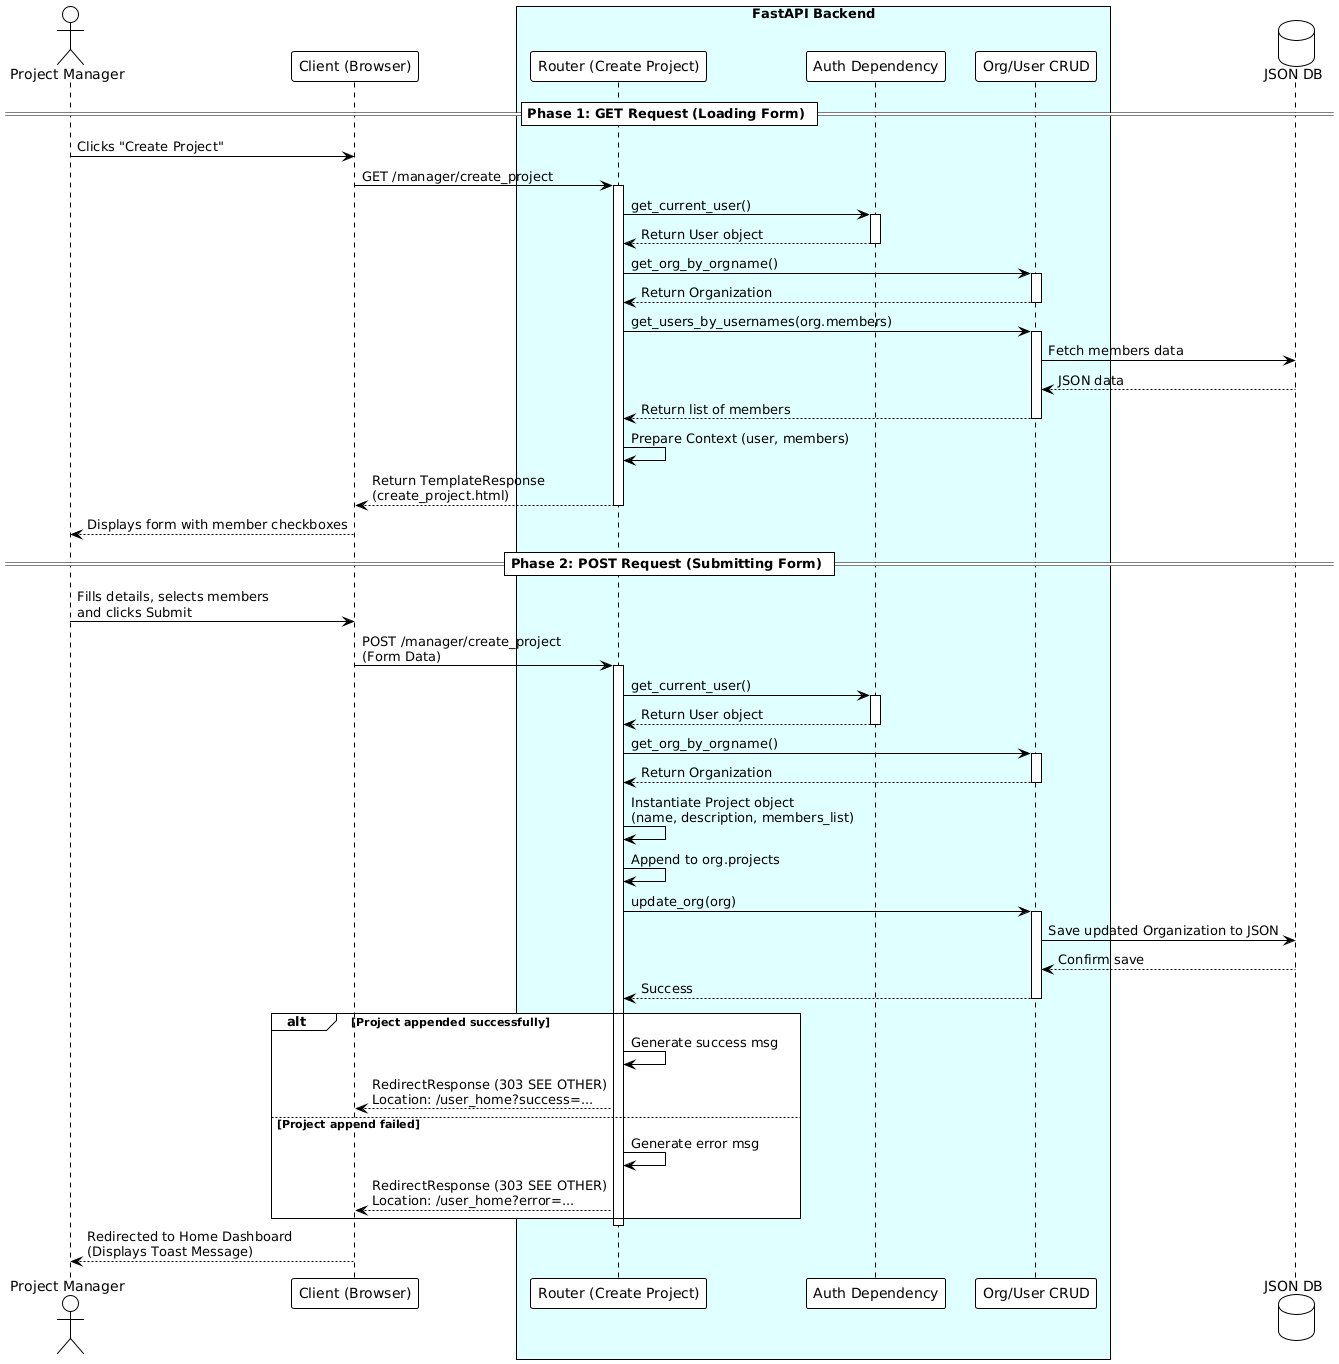
\includegraphics[width=1\linewidth]{images/sequence_diagram_project_creation.png}
    \caption{Sequence Diagram: Project Creation}
\end{figure}

\subsection{Profile}
The Profile section acts as the personal hub for the user, centralizing account 
settings, competence tracking, and career development tools.

\subsubsection{Target Roles and Skills Management}
Both employees and managers can access this area to view their personal data and 
securely change their passwords. More importantly, users can manage their professional 
portfolio by viewing, adding, or removing their personal skills and desired target 
roles. To streamline the data entry process, the platform supports bulk operations: 
users can download a standardized CSV template directly from the profile interface, 
enabling the simultaneous upload of multiple skills. Furthermore, the dashboard 
provides a direct link to the external \textit{MuchSkills} platform, serving as an 
auxiliary tool to help users intuitively map and build their personal competence 
profile before importing it into the system.

If a user is currently affiliated with an organization, a dedicated subsection 
displays their ``organizational skills''---competencies that are directly assigned 
and managed by the company. Through this interface, users also retain the autonomy 
to officially leave their current organization if needed.

\subsubsection{Cedefop Forecast and Skill Gap Evaluation}
Once a user has defined their current skill set and selected one or more target roles, 
the platform can perform a comprehensive skill gap analysis. The system compares the 
user's existing competencies against the specific requirements of the desired roles,
highlighting areas for improvement. Additionally, the application retrieves Cedefop 
forecast data related to these target roles, offering the user valuable insights 
into future labor market trends, job demand, and employment projections.

\subsubsection{Course Recommendation}
Based on the exact skill gaps identified in the previous step, the platform provides 
customized educational suggestions. This recommendation engine---which is the same core 
logic utilized in the Project Manager dashboard---analyzes the missing 
competencies and cross-references them with available training resources. 
By doing so, the system generates a highly personalized learning path, proposing 
the most relevant courses to help the user efficiently bridge the gap between their 
current capabilities and their professional goals. 

To facilitate offline review and long-term career planning, users can 
conveniently export the complete analysis---including the skill 
gap results and course recommendations---into a consolidated PDF report.

\begin{figure}[htbp]
    \centering
    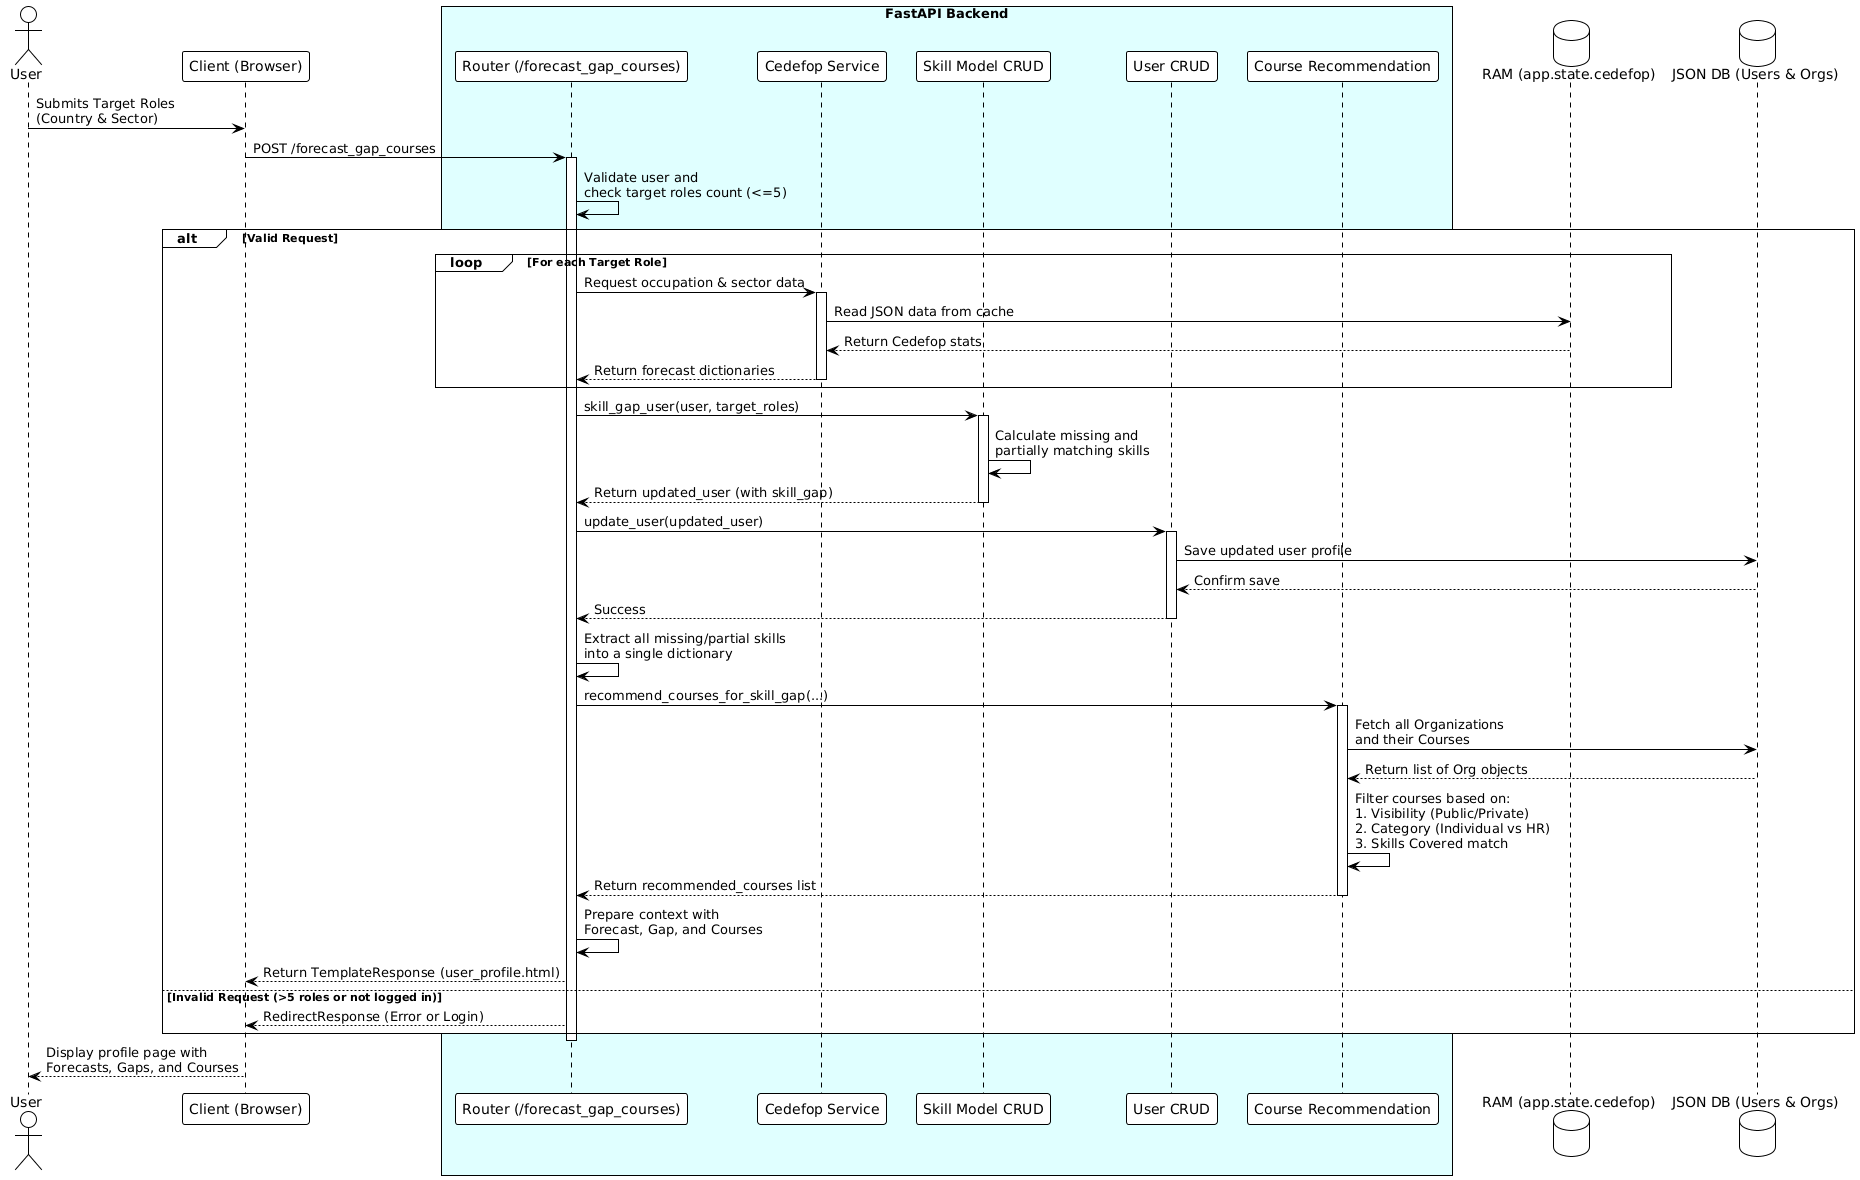
\includegraphics[width=1\linewidth]{images/sequence_diagram_forecast_gap_course.png}
    \caption{Sequence Diagram: Cedefop's Forecast, Skill Gap and Course Recommendation}
\end{figure}

\newpage

\section{Organization Features}
This section details the functionalities available to Organization accounts. 
Unlike individual users who focus on personal career development, an Organization 
profile represents the company as a whole. Its primary purpose is to oversee the 
workforce, manage internal training resources, and analyze competence gaps at a macro 
level, providing an administrative overview of the company's human resources.

\subsection{Home}
The Home dashboard for an organization is designed to provide a high-level summary 
of ongoing activities, focusing primarily on project monitoring.

\subsubsection{Projects}
Through this interface, the organization can access a comprehensive list of all 
active projects currently overseen by its internal Managers. It is important to note 
that this is a strictly read-only view: the organization can monitor the status, but 
the direct management, creation, and modification of the projects remain the sole 
responsibility of the delegated Managers.

\subsection{Profile}
The Profile area serves as the central administrative hub for the organization, 
allowing the management of account credentials, personnel, and proprietary training 
materials. As with individual users, this section also includes basic settings to 
view corporate data and securely update the account password.

\subsubsection{Team Members}
The organization can view its current workforce, distinguishing between standard 
employees and managers. To expand the team, the organization can send an official 
invitation by entering a specific username into the recruitment form, facilitated 
by a comprehensive list of all registered platform users. The invited user then 
retains the autonomy to accept or decline the request. Furthermore, the organization 
holds the authority to adjust user privileges within the company, allowing them to 
promote standard employees to the Manager role or demote them as organizational 
needs dictate. In addition, the platform provides a 
direct link to the external \textit{MuchSkills} platform. 
This allows the organization to design a comprehensive skill model for 
its workforce and seamlessly integrate these profiles into the system via 
a bulk CSV import.

\begin{figure}[htbp]
    \centering
    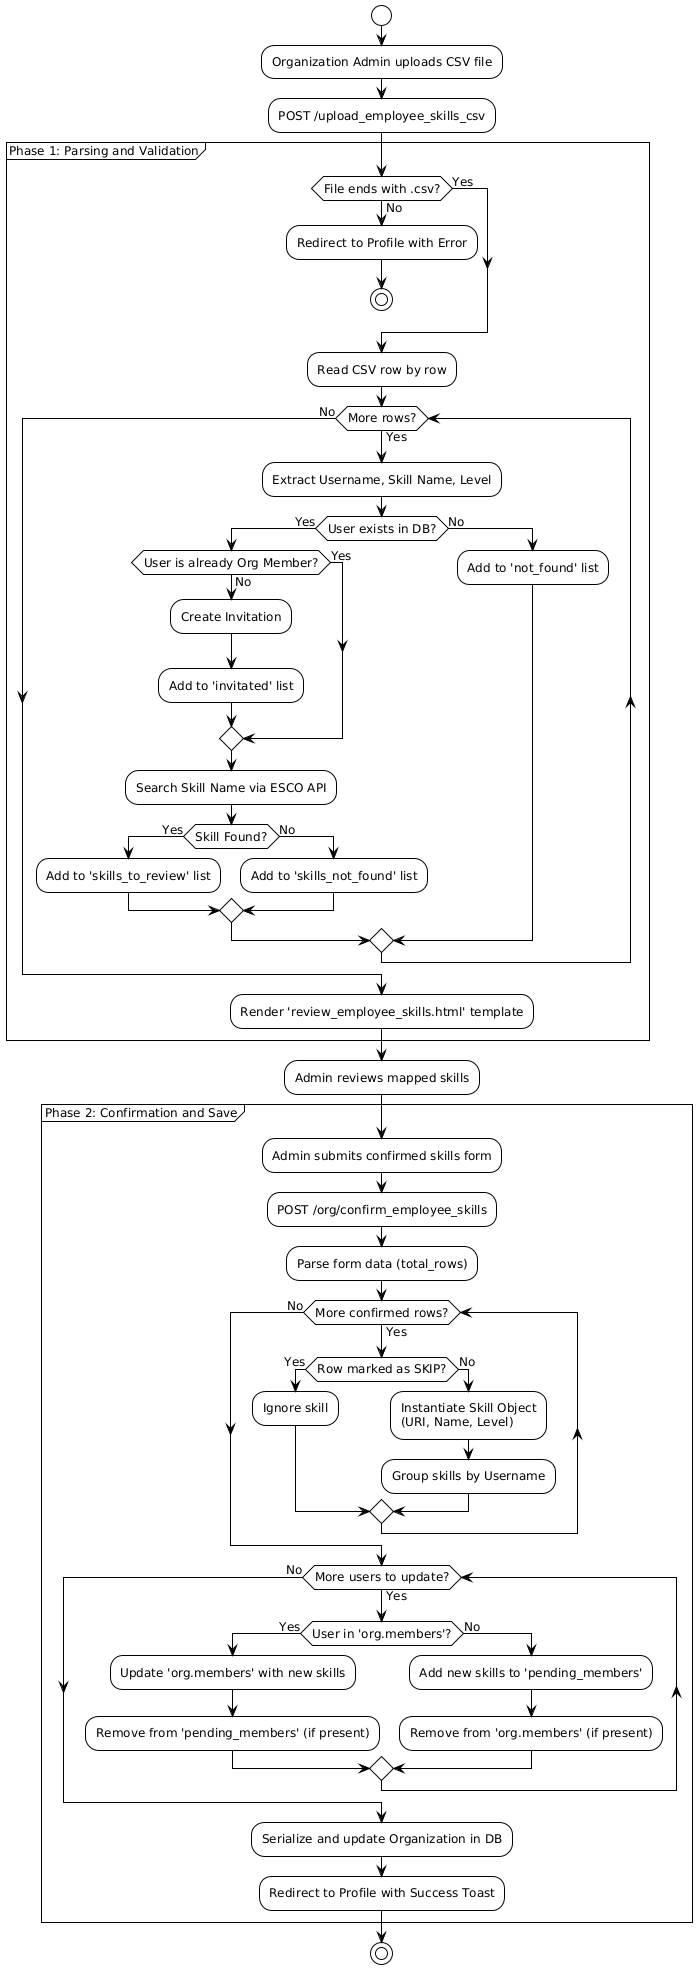
\includegraphics[width=0.52\linewidth]{images/activity_diagram_org_upload_confirm_skills.png}
    \caption{Activity Diagram: CSV Upload and Skill confirmation}
\end{figure}

\subsubsection{Global Skill Gap Evaluation}
Provided the organization has active projects, it can perform a macroscopic 
\mbox{analysis} of its workforce capabilities. Instead of evaluating a single 
user, this feature calculates a global skill gap by comparing the aggregated 
competencies of the current employees against the collective requirements of 
the ongoing projects. Based on these company-wide deficiencies, the platform 
suggests HR-oriented courses. These specific recommendations are designed for 
strategic corporate upskilling and human resource planning, rather than individual 
learning paths. Similar to the functionality available to individual users, 
organizations can export this comprehensive evaluation into a consolidated PDF 
report, facilitating offline review and strategic decision-making 
at the management level.

\subsubsection{Courses Management}
The platform allows organizations to act as educational providers by creating 
and distributing their own training modules. Through this interface, the company 
can view a complete catalog of its authored courses, seamlessly create new ones, 
and edit or delete existing materials. A critical feature of this management tool 
is the visibility toggle: courses can be published as ``public'' to be accessible 
by any user on the platform, or set to ``private,'' ensuring that only the 
organization's officially affiliated employees can view and benefit from them.

\begin{figure}[htbp]
    \centering
    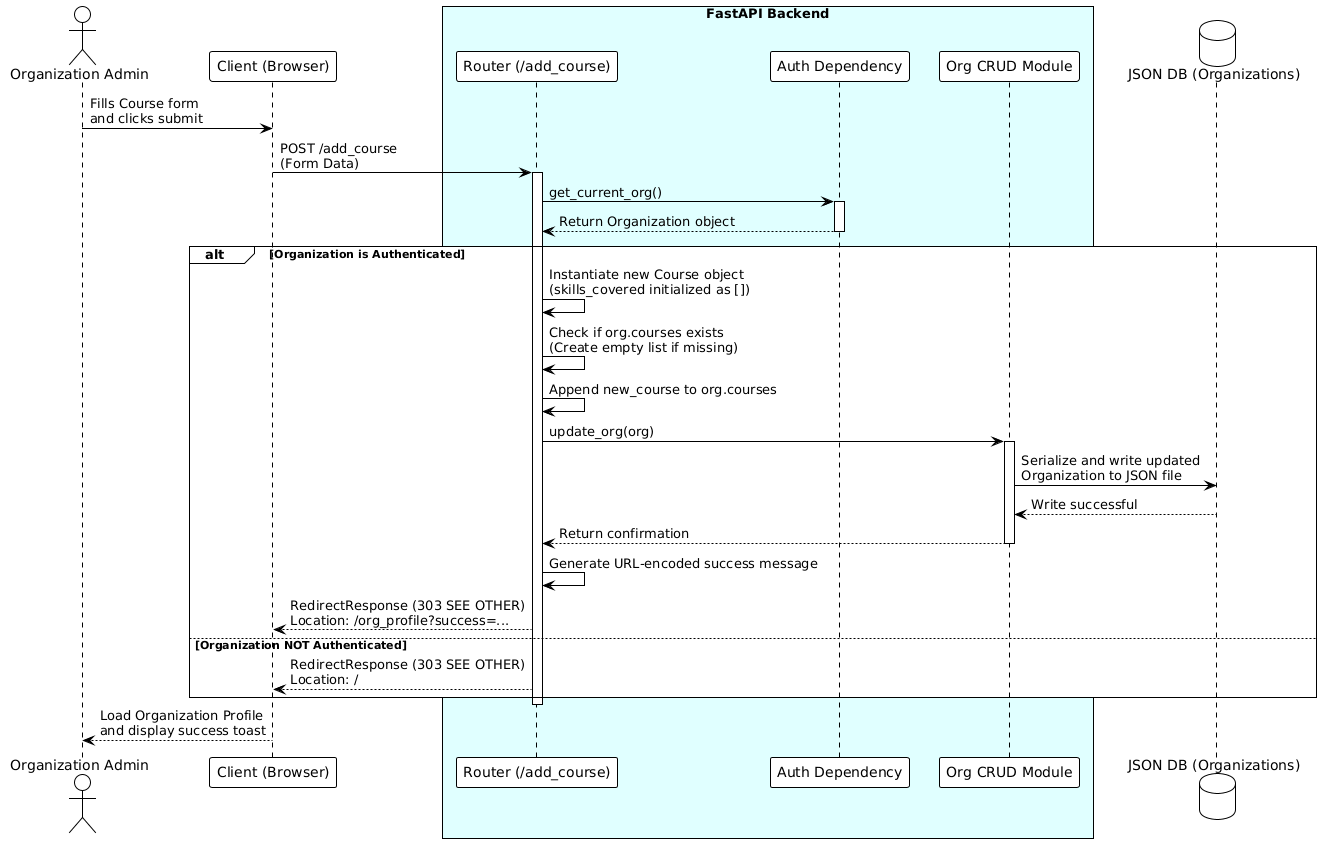
\includegraphics[width=1\linewidth]{images/sequence_diagram_org_create_course.png}
    \caption{Sequence Diagram: Course Creation}
\end{figure}

\section{Guest Features}
The platform also accommodates unregistered users by providing a restricted ``Guest'' 
access mode. For individuals who prefer not to create a formal account, the system 
offers a streamlined interface to explore the core competency catalog. Through this 
guest portal, users can perform basic searches for professional roles and individual 
skills, which are directly powered by the ESCO API. 

However, compared to registered employees or organizations, this browsing experience 
is intentionally synthesized and limited in scope. Guests can view roles 
of the queried terms, but they cannot access 
advanced, stateful features such as profile creation, skill gap evaluation, or 
personalized course recommendations. This approach allows external users to evaluate 
the platform's core search capabilities while maintaining data privacy and 
encouraging formal registration for full access.

\newpage

\section{ESCO API Integration}
A core component of the platform is the integration with the ESCO API, hosted by 
the European Commission. The system interacts with this external service using the 
Python \texttt{requests} library to fetch standardized data regarding professional 
roles and specific skills.

The backend implements dedicated functions to query the API for single role 
details (including the ISCO classification code and essential skills), 
as well as search functions to retrieve lists of occupations or skills based 
on user input. For instance, the system requests the \texttt{hasEssentialSkill} 
relation from the API to automatically map the necessary competencies for a given 
job title. The JSON responses provided by the API are subsequently parsed and 
converted into internal \texttt{Role} and \texttt{Skill} data models to be utilized 
by the application's business logic.

\section{Data Management}
Given the platform's reliance on extensive datasets, particularly for the Cedefop 
employment forecasts, efficient data management was a priority. The original Cedefop 
data, initially provided in Excel format, was converted into structured JSON files. 

To ensure high performance and minimize read operations from the disk during 
execution, the application utilizes the FastAPI \texttt{app.state} object. 
Upon server startup, the system loads these JSON files directly into the server's RAM. 
This in-memory caching strategy significantly reduces the latency when users calculate 
skill gaps and request forecast data, allowing the application to respond to these 
computationally heavy requests almost instantaneously. User and organization data, 
as well as active invitations, are also managed via JSON-based local databases, 
allowing for a lightweight and easily deployable architecture.

\subsection{Database Schema}
While the platform does not use a traditional relational database, its 
schema is explicitly defined 
and validated using Python \texttt{Pydantic} models. This approach ensures strict 
typing, data validation, and rapid serialization/deserialization when interacting 
with the JSON files. 
The complete database schema is centrally defined within the \texttt{app/models.py} 
file of the project's source code. The primary entities structuring the platform are:

\begin{itemize}
    \item \textbf{Skill and Role:} These are the foundational building blocks of 
    the platform, designed to perfectly mirror the data structure retrieved from 
    the external ESCO API. 
    \item \textbf{User Model:} Stores individual credentials, assigned roles 
    (defined by the \texttt{UserLevel} Enum), and organizational affiliation. 
    It relies heavily on nested data, storing the user's personal portfolio 
    in the \texttt{individual\_skills} array, alongside the selected 
    \texttt{target\_roles} and the dynamically calculated \texttt{skill\_gap} 
    objects.
    \item \textbf{Organization Model:} Represents corporate entities. It 
    contains the organization's credentials and dynamically embeds comprehensive 
    lists of authored \texttt{courses} and internal \texttt{projects}. 
    Workforce mapping is ingeniously handled via dictionaries (\texttt{members} 
    and \texttt{pending\_members}), mapping string usernames directly to their 
    respective arrays of \texttt{Skill} objects.
    \item \textbf{Project and Course Models:} Embedded within the Organization 
    model, the \texttt{Project} tracks the \texttt{manager}, 
    \texttt{assigned\_members}, and specific \texttt{target\_roles}. 
    The \texttt{Course} model tracks detailed metadata (e.g., \texttt{ects}, 
    \texttt{category}, \texttt{cost}) and the \texttt{skills\_covered} required 
    for the recommendation engine. The generation of unique identifiers is 
    automated using the \texttt{uuid4} standard.
    \item \textbf{Invitation Model:} An independent structure that manages 
    the asynchronous flow of adding users to organizations, tracking the 
    \texttt{orgname}, \texttt{username}, and the \texttt{status} (pending, 
    accepted, declined) of the request.
\end{itemize}

\subsection{Main Queries and Data Processing Logic}
Given this file-based and in-memory architecture, data retrieval does not rely 
on standard SQL statements. 
Instead, ``queries'' are implemented as optimized Python CRUD (Create, Read, 
Update, Delete) operations that interact with the in-memory data structures or 
JSON files.
The principal query mechanisms and algorithmic logic utilized by the system include:

\begin{itemize}
    \item \textbf{Direct File I/O (CRUD Operations):} Modules like 
    \texttt{crud\_user.py} and \texttt{crud\_org.py} manage persistent 
    storage by mapping objects to physical JSON files. Unique identifiers, 
    such as the \texttt{username} or \texttt{orgname}, act as primary keys 
    to construct file paths (e.g., \texttt{data/users/\{username\}.json}). 
    Updates are performed securely by serializing the Pydantic models back 
    into the file system using \texttt{model\_dump\_json()}.
    
    \item \textbf{Relational Mapping and Aggregation:} To emulate SQL 
    \texttt{JOIN} operations, the system uses aggregation functions. 
    For instance, \texttt{get\_users\_by\_usernames} iteratively queries 
    the file system to resolve an array of string usernames into a fully 
    populated list of \texttt{User} objects. This is vital for the Project 
    Manager dashboard to visualize team members.
    
    \item \textbf{Skill Gap Algorithmic Queries:} The \texttt{crud\_skill\_models.py} 
    module executes the most computationally intensive ``queries''.  To optimize 
    performance, the algorithm first flattens the user's current competencies into 
    a hash map (\texttt{user\_skills\_dict}), enabling O(1) time complexity lookups 
    via the skill URI. The mathematical engine then evaluates the gap: a fully 
    possessed skill grants $1.0$ point, whereas partially matched skills calculate 
    a fractional score based on the ratio of the user's level versus the required 
    level (\texttt{user\_level / req\_level}). The output categorizes skills into 
    \texttt{matching}, \texttt{partially\_matching}, and \texttt{missing} arrays.
    
    \item \textbf{In-Memory Navigation (Cedefop Data):} The \texttt{cedefop\_read.py} 
    module handles data extraction from the Cedefop JSON loaded entirely into the 
    server's RAM during startup. Instead of disk reads, it utilizes nested 
    dictionary \texttt{.get()} methods chained together. The module features 
    smart parsing logic: it dynamically slices the incoming ISCO code string 
    to navigate the correct hierarchical depth of the dataset, such as extracting 
    the first two digits (\texttt{isco\_clean[:2]}) to query sector employment 
    details or qualifications.
\end{itemize}

\newpage

\section{Testing and Quality Assurance}
To guarantee the stability and reliability of both the backend calculations and the 
frontend endpoints, a comprehensive testing suite was implemented using the 
\textbf{pytest} framework. The testing strategy covers HTML route rendering, 
internal backend logic (such as the skill gap evaluation algorithms), and proper 
HTTP status code responses.

To simulate client interactions without requiring a live server, the FastAPI 
\texttt{TestClient} is utilized. Furthermore, to isolate the testing environment 
and prevent the corruption of actual production data, the system employs the 
\mbox{\texttt{monkeypatch}} utility provided by pytest. This allows the automatic 
generation of temporary, isolated JSON directories for users, organizations, 
and invitations during the testing phase, which are automatically 
discarded upon completion. 

The following snippet illustrates the configuration of the unified mocking database 
used across the test suite:

\begin{lstlisting}[caption={Pytest configuration with TestClient and temporary mock databases}]
import pytest
from fastapi.testclient import TestClient
from app.main import app
from app.crud import crud_user, crud_org

@pytest.fixture(scope="module")
def client():
    with TestClient(app) as c:
        yield c

@pytest.fixture(autouse=True)
def mock_database(tmp_path, monkeypatch):
    # Create temporary directories
    temp_users_dir = tmp_path / "test_users"
    temp_orgs_dir = tmp_path / "test_orgs"
    temp_inv_dir = tmp_path / "test_invitations"
    
    temp_users_dir.mkdir(exist_ok=True)
    temp_orgs_dir.mkdir(exist_ok=True)
    temp_inv_dir.mkdir(exist_ok=True)

    # Forcing code to use new tmp dirs
    monkeypatch.setattr(crud_user, "DATA_DIR_USERS", str(temp_users_dir))
    monkeypatch.setattr(crud_user, "DATA_INV_DIR", str(temp_inv_dir))

    monkeypatch.setattr(crud_org, "DATA_DIR_ORGS", str(temp_orgs_dir))
    monkeypatch.setattr(crud_org, "DATA_INV_DIR", str(temp_inv_dir))

    yield
\end{lstlisting}

\end{document}